\documentclass[tikz,border=2pt]{standalone}
\usepackage{amsmath}
\usepackage{pgfplots}
\pgfplotsset{compat=1.18}
\usetikzlibrary{arrows.meta}
\begin{document}
% Payment Y = min((X-d)_+, u) with d = 100, u = 500: zero up to 100, slope 1 up to d+u = 600, then capped at 500;
% a loss of 800 is paid 500, while a ground-up cap of 500 would pay min(X,500) - 100 = 400.
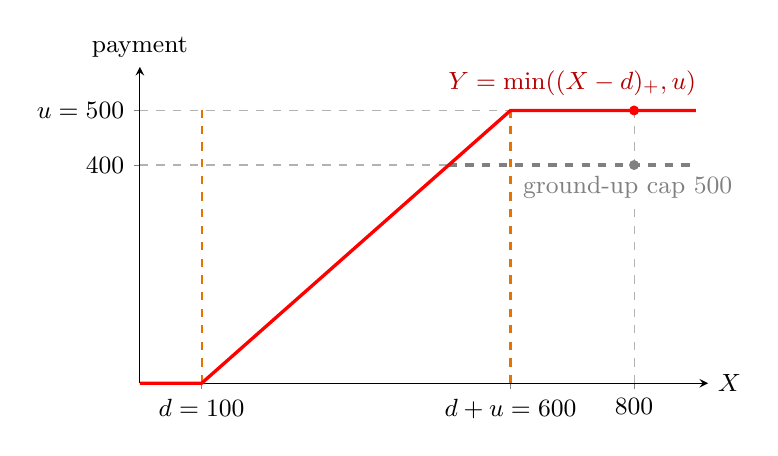
\begin{tikzpicture}[font=\small, >={Latex[length=2mm]}]
  \begin{axis}[
    axis lines=left, xmin=0, xmax=920, ymin=0, ymax=580,
    xtick={100,600,800}, xticklabels={$d=100$,$d+u=600$,$800$}, ytick={400,500}, yticklabels={$400$,$u=500$},
    xlabel={$X$}, ylabel={payment},
    xlabel style={at={(axis description cs:1,0)}, anchor=west},
    ylabel style={rotate=-90, at={(axis description cs:0,1)}, anchor=south},
    width=8.8cm, height=5.6cm, clip=false]
    \draw[orange!90!black, thick, dashed] (axis cs:100,0) -- (axis cs:100,500);
    \draw[orange!90!black, thick, dashed] (axis cs:600,0) -- (axis cs:600,500);
    \draw[gray!60, thin, dashed] (axis cs:800,0) -- (axis cs:800,500);
    \draw[gray!60, thin, dashed] (axis cs:0,400) -- (axis cs:500,400);
    \draw[gray!60, thin, dashed] (axis cs:0,500) -- (axis cs:600,500);
    \draw[gray, very thick, dashed] (axis cs:500,400) -- (axis cs:900,400);
    \draw[red, very thick] (axis cs:0,0) -- (axis cs:100,0) -- (axis cs:600,500) -- (axis cs:900,500);
    \fill[red] (axis cs:800,500) circle (1.8pt);
    \fill[gray] (axis cs:800,400) circle (1.8pt);
    \node[red!70!black, anchor=south] at (axis cs:700,510) {$Y=\min((X-d)_+,u)$};
    \node[gray, anchor=north west, fill=white, inner sep=1pt] at (axis cs:615,385) {ground-up cap $500$};
  \end{axis}
\end{tikzpicture}
\end{document}
